\clearpage
\appendix

\section{The LSST Baseline Design}

The following tables includes excerpts from the March 16, 2010 LSST Baseline
Design Summary (available from http://www.lsst.org/lsst/science/survey\_requirements)
that are most relevant to this document.

\begin{table}[h]
\centerline{\large Excerpts from the Baseline Design Summary}
\centerline{
\begin{tabular}{|l|l|}
\hline
   Quantity                &     Baseline Design Specification     \\
\hline
Optical Configuration      &  3-mirror modified Paul-Baker          \\
Mount configuration        &  Alt -- Azimuth                        \\
Final f-Ratio              &  f/1.234                                \\
Field of view area         &  9.6 deg$^2$                           \\
Aperture                   &  8.4 m                                 \\
Effective aperture         &  6.68 m                                \\
Effective \'etendue (A$\Omega$)  &  319 m$^2$deg$^2$                \\
Plate Scale                &  50.9 microns/arcsec (0.2 arcsec pix)  \\
Pixel count                &  3.2 Gigapixel                         \\
Wavelength Coverage        &  330 -- 1070 nm                        \\
Standard exposure sequence &  41 sec total for 2x15 sec exposure    \\
                           &  (with slew, without filter change)    \\
\hline
\end{tabular}
}
\caption{The LSST March 2010 Baseline Design Parameters.}
\end{table}

\clearpage
\section{The Universal Cadence Strategy}

Strict optimization of each of the numerous science programs that LSST will
enable would certainly result in the same number of observing strategies.
However, thanks to the large \'{e}tendue, it is possible to design a universal
cadence that would result in a common database of observations to be used by
all science programs. An example of such a cadence is described here and
presented as a ``proof of concept'' rather than as a specific requirement
on the observing strategy. It does not address the possibility of deeper,
or more frequent, KBO and SNe surveys discussed in \S 3.4.

This, so-called ``universal cadence'', has a number of desirable properties,
and in particular, samples a wide range of time scales that are necessary for
time domain science. Equally important, the proposed cadence is invariant to
time translation and reversal, a feature that is desirable for a massive
steady-state synoptic sky survey. More details about this proposal are available
in the LSST Science Working Group report, and here only its essential
characteristics are described.

The strategy proposes two revisits closely separated in time (15-60 min)
to enable a robust and simple method for linking main-belt asteroids (MBA).
Their sky surface density is about two orders of magnitude higher than the
expected density of potentially hazardous asteroids (PHA), and thus MBAs
must be efficiently and robustly recognized in order to find PHAs. MBAs
move about 3-18 arcmin in 24 hours, which is larger than their typical
nearest neighbor distance at the depths probed by LSST (2.3 arcmin on the
Ecliptic). Two visits closely separated in time enable linking based on
a simple search for the nearest moving neighbor, with a false matching
rate of only a few percent.

With this cadence, it is possible to observe 20,000 $deg^2$ of sky
in about three nights, with two visits per field. The colors of
transients (such as SNe) and moving objects can also be measured by
using two different filters for the two visits (with a preference given
to the $r$ band).

Due to the proposed overlap between successive fields of view, about
17\% of the observed area represent multiple observations with a variety
of time scales. With a representative choice of various free parameters,
about 5\% of the observed area would be revisited within 25 sec.
Another 10\% of the area would be reobserved with a fairly uniform
sampling of time scales ranging from 25 sec to 15 min.

\clearpage
\section{The LSST Bandpasses}

\begin{figure}[h]\centering
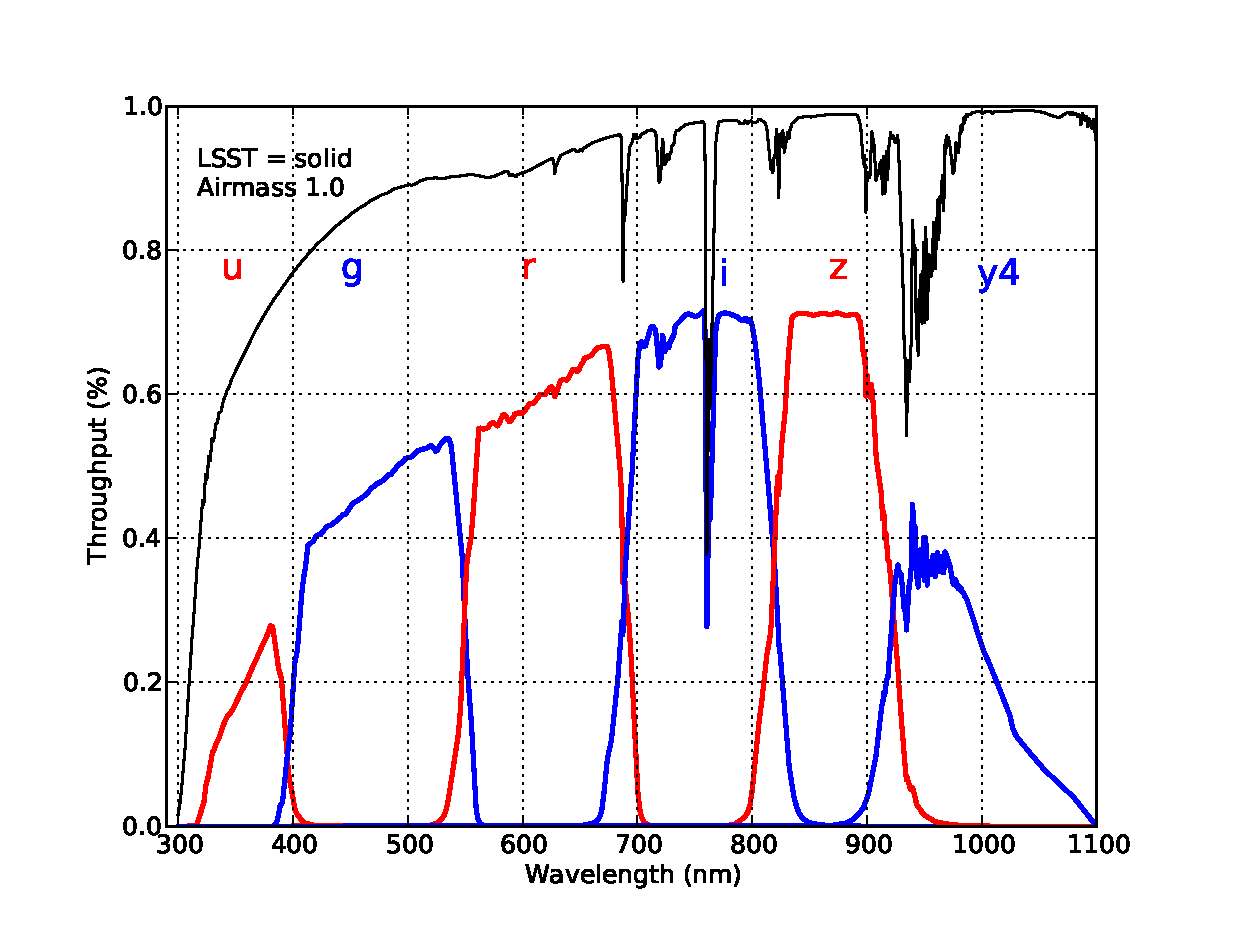
\includegraphics[width=\textwidth]{filters_thruputs}
\caption{The \textit{current} design of the LSST bandpasses (thick lines:
the full throughput, including the atmosphere and idealized system,
described by $S_b(\lambda)$ from eq.~\ref{SDef}).
The thin line shows the throughput for a standard atmosphere at
airmass $X=1.0$ used in computations ($S^{atm}(\lambda)$ from eq.~\ref{SDef}).}
\end{figure}


\clearpage
\section{The Seeing Distribution at the Cerro Pach\'{o}n site}

\begin{figure}[h!]\centering
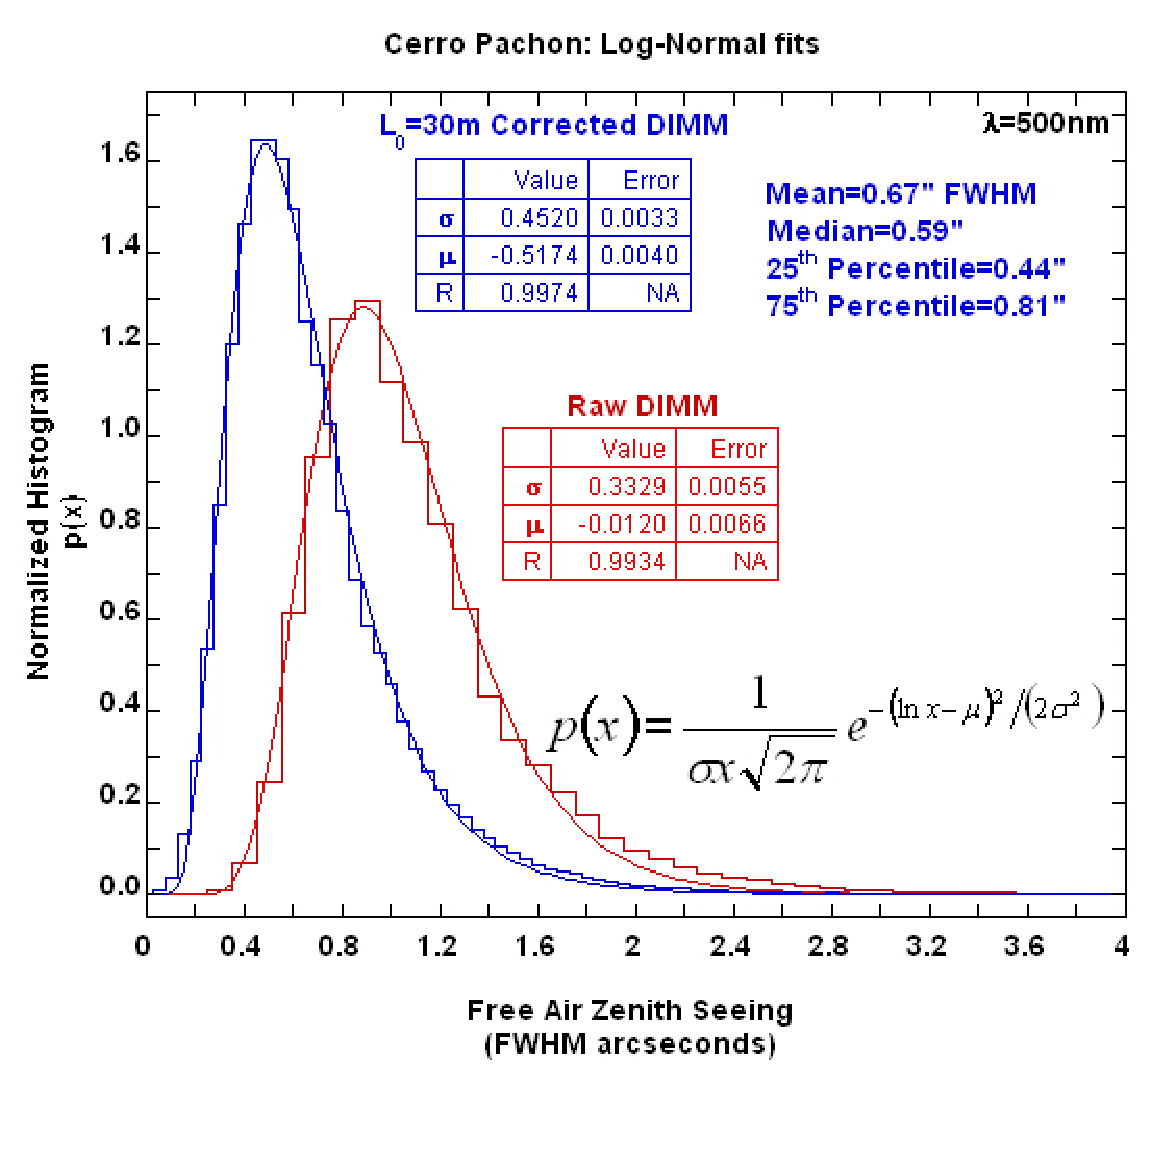
\includegraphics[width=13cm]{CerroPachonSeeing}
\caption{The seeing distribution measured at the Cerro Pach\'{o}n site using DIMM at
500 nm (red histogram), and corrected using the outer scale parameter of 30 m
(blue histogram). For details about the outer scale correction see Tokovinin
2002 (PASP, 114, 1156). The lines show best-fit log-normal distributions, with
the best-fit parameters as shown in the inset (computed by C. Claver).}
\end{figure}




\clearpage
\section{The Document History}

\begin{enumerate}
\item \textbf{Version 4.3 (September 2007)} The first version approved by the LSST Board, placed under the Change
 Control Board, and made public.

\item \textbf{Version 5.1 (May 2010)} The most important changes, relative to v4.3, are:
\begin{itemize}
\item Incorporated references to the LSST Science Book
\item Made listed science drivers normative
\item Listed expected performance for photometric redshifts of galaxies
\item Improved quantitative drivers and specifications for trigonometric parallax and proper motion
\item Adopted a general principle that software algorithms should not dominate measurement errors
\item Relaxed minimum requirements for single-image depth (by 0.2-0.3 mag)
\item Made it explicit that the system throughput function is a part of photometric data products
\item Removed specifications for ghosting
\item Removed specifications for modeling residuals for single-image ellipticity
\item Added specification for time-recording accuracy
\item Made explicit mini and micro surveys
\item Made explicit the three levels of data products
\end{itemize}

\item \textbf{Version 5.2 (June 2011)} The most important changes, relative to v5.1, are:
\begin{itemize}
\item Added the first paragraph in section ``Galaxy shear measurement accuracy, and PSF ellipticity residuals''
          (see Table 27).
\item Added requirements for the image processing software in Section 3.5.
\item Updated Science Council membership list.
\end{itemize}

\end{enumerate}
